% This work is licensed under the Creative Commons
% Attribution-NonCommercial-ShareAlike 4.0 International License. To view a copy
% of this license, visit http://creativecommons.org/licenses/by-nc-sa/4.0/ or
% send a letter to Creative Commons, PO Box 1866, Mountain View, CA 94042, USA.
% (c) Eric Kunze, 2020
%%%%%%%%%%%%%%%%%%%%%%%%%%%%%%%%%%%%%%%%%%%%%%%%%%%%%%%%%%%%%%%%%%%%%%%%%%%%%%%
% Template for exercises and homework at TU Dresden.
%%%%%%%%%%%%%%%%%%%%%%%%%%%%%%%%%%%%%%%%%%%%%%%%%%%%%%%%%%%%%%%%%%%%%%%%%%%%%%%

\documentclass[ngerman, a4paper, 11pt]{article}

\usepackage[ngerman]{babel}
\usepackage[top=2.5cm,bottom=2.5cm,left=2.5cm,right=2.5cm]{geometry}

\usepackage{parskip}    % split paragraphs by vspace instead of intendations
\usepackage[onehalfspacing]{setspace} % increase row-space

\usepackage{xifthen}
\usepackage{xparse}

%%%%%%%%%%%%%%%%%%%%%%%%%%%%%%%%%%%%%%%%%%%%%%%%%%%%%%%%%%%%%%%%%%%%%%%%%%%%%%%
% SCHRIFTEN
\usepackage[utf8]{inputenc}
\usepackage{chngcntr}
\usepackage{eufrak}

\usepackage{lmodern}
\usepackage[normalem]{ulem}

\usepackage[autostyle=true,english=british]{csquotes}

% new font OpenSans
\usepackage[scale=1]{opensans}
\newcommand*{\osfamily}{\fontfamily{fos}\selectfont}
\DeclareTextFontCommand{\textos}{\osfamily}

\usepackage{listings}

%%%%%%%%%%%%%%%%%%%%%%%%%%%%%%%%%%%%%%%%%%%%%%%%%%%%%%%%%%%%%%%%%%%%%%%%%%%%%%%
% EIGENSCHAFTEN
\newcommand{\name}{Eric Kunze}
\newcommand{\matnr}{4679202}
\newcommand{\email}{\href{mailto:eric.kunze@mailbox.tu-dresden.de}{\ttfamily eric.kunze@mailbox.tu-dresden.de}}

\newcommand{\modul}{Versicherungsmathematik -- Risikomodelle}
\newcommand{\semester}{Wintersemester 2020/21}

%\renewcommand{\tutor}{TUTOR}
%\renewcommand{\gruppe}{Tag x. DS, (un)gerade Woche}

\newcommand{\professor}{Prof. Dr. Martin Keller-Ressel}
\newcommand{\fakultaet}{Mathematik}
\newcommand{\institut}{Stochastik}
\newcommand{\lehrstuhl}{Stoch. Analysis \& Finanzmathematik}

%%%%%%%%%%%%%%%%%%%%%%%%%%%%%%%%%%%%%%%%%%%%%%%%%%%%%%%%%%%%%%%%%%%%%%%%%%%%%%%
% GRAPHICS
\usepackage{graphicx}
\usepackage[table,dvipsnames]{tudscrcolor} % package xcolor loaded automatically
\usepackage[font=small,labelfont=bf]{caption} % captions of non-floated figures

\usepackage[most]{tcolorbox}

\usepackage{tikz}
\usetikzlibrary{matrix, patterns,arrows,calc,decorations.pathmorphing,backgrounds, positioning,fit,petri,decorations.fractals}
\usepackage{pgf}
\usepackage{pgfplots}
\pgfplotsset{compat=1.10}   % in my packages used compat=1.15
\usepgfplotslibrary{fillbetween}

% tabulars
\usepackage{tabularx}   % tabularx-environment (explicitly set width of columns)
\usepackage{multirow}
\usepackage{booktabs}   % improved rules

%%%%%%%%%%%%%%%%%%%%%%%%%%%%%%%%%%%%%%%%%%%%%%%%%%%%%%%%%%%%%%%%%%%%%%%%%%%%%%%
% ENUMERATIONS
\usepackage{enumerate}
\usepackage[inline]{enumitem}       % customize label

\renewcommand{\labelitemi}{\raisebox{1pt}{\scalebox{.4}{$\blacksquare$}}}
\renewcommand{\labelitemii}{$\vartriangleright$}
\renewcommand{\labelitemiii}{--}
% Variantionen des Dreiecks als Aufzählungszeichen $\blacktriangleright$ / $\vartriangleright$ / $\triangleright$

\renewcommand{\labelenumi}{(\arabic{enumi})}
\renewcommand{\labelenumii}{\alph{enumii}.}
\renewcommand{\labelenumiii}{\roman{enumiii}.}

%%%%%%%%%%%%%%%%%%%%%%%%%%%%%%%%%%%%%%%%%%%%%%%%%%%%%%%%%%%%%%%%%%%%%%%%%%%%%%%
% PAGE LAYOUT
\usepackage{scrlayer-scrpage}
\clearpairofpagestyles
\newpairofpagestyles[scrheadings]{firstpage}{\ohead*{}\cfoot*{\pagemark}}
\newpairofpagestyles[scrheadings]{normalpage}{
    \ihead*{\fosfamily\color{cdgray}\small\modul}
    \ohead*{\fosfamily\color{cdgray}\small\name~ (\matnr)}
    \cfoot*{\pagemark}}

\pagestyle{normalpage}
\pagenumbering{arabic}

%%%%%%%%%%%%%%%%%%%%%%%%%%%%%%%%%%%%%%%%%%%%%%%%%%%%%%%%%%%%%%%%%%%%%%%%%%%%%%%
% TITLEPAGE
\newcommand{\makeTUtitle}[1][]{%
    \begin{titlepage}
        \pagecolor{cddarkblue!90} \color{white}%
        \raggedright \fosfamily%
        \setlength{\parindent}{0pt}%
    % Logo / Kopf
        \hspace{-18.6mm} %
        
\includegraphics[scale=0.6]{TUD-white.pdf} \\
        \vspace{3mm}
        \begin{tabular}{m{\textwidth}}
            \hline
            \hspace{-4pt}\small{\textbf{Fakultät \fakultaet} Institut für \institut, Professur für \lehrstuhl} \\
            \hline
        \end{tabular} \\
    % Titel
        \vspace{5cm}
        {\Huge\bfseries \MakeUppercase \modul \par}
        \vspace{0.5cm}%
        {\Large \itshape Übungen} \\%
        \vspace{1.5cm}
        \textbf{{\Large \professor}} \par
        \vspace{0.5cm}
        {\large \semester}
    % Fußzeile
        \vfill%
        \begin{tabular}{lll}
            Autor  & : & \name \\
            E-Mail & : & \email \\
        \end{tabular}%
    \end{titlepage}
    \nopagecolor
}

%%%%%%%%%%%%%%%%%%%%%%%%%%%%%%%%%%%%%%%%%%%%%%%%%%%%%%%%%%%%%%%%%%%%%%%%%%%%%%%
% COUNTER
\usepackage{chngcntr}

\newcounter{taskcount}
\newcounter{blattcount}
\newcounter{thmcount}

\counterwithin{page}{blattcount}
\counterwithin{equation}{blattcount}
\counterwithin{figure}{blattcount}
\counterwithin{table}{blattcount}

% automatic reset of task counter in each blatt
%\pretocmd{\exercisePage}{\setcounter{taskcount}{0}}{}{}

%\counterwithin{taskcount}{blattcount}

%%%%%%%%%%%%%%%%%%%%%%%%%%%%%%%%%%%%%%%%%%%%%%%%%%%%%%%%%%%%%%%%%%%%%%%%%%%%%%%
% EXERCISE PAGE
\newcommand{\header}{%
        {\fosfamily%
            \fcolorbox{cddarkblue}{cdblue!20}{%
                \begin{minipage}{\dimexpr0.74\linewidth-\fboxrule-\fboxsep}
                    {\huge \textbf{Hausaufgaben}} \vspace{3pt} \\
                    \textbf{\modul} -- Übungsblatt \theblattcount
                \end{minipage}%
                \begin{minipage}{\dimexpr0.24\linewidth-\fboxrule-\fboxsep}
                    \flushright \textbf{\name} \\
                    Matr.-Nr. \matnr
                \end{minipage}%
        }}%
    }%

\NewDocumentEnvironment{exercisePage}{O{}}{%
    \pagebreak%
    \stepcounter{blattcount} \setcounter{page}{1}%
    \thispagestyle{firstpage}
    \header \\[6pt]
    \setcounter{figure}{0}
    \setcounter{equation}{0}%
    \setcounter{table}{0}%
    \setcounter{thmcount}{0}
    %
    \ifthenelse{\isempty{#1}}{}{%
        {\fosfamily \itshape Thema: #1} \par%\\[12pt]%
    }
}{}

%%%%%%%%%%%%%%%%%%%%%%%%%%%%%%%%%%%%%%%%%%%%%%%%%%%%%%%%%%%%%%%%%%%%%%%%%%%%%%%
% MATH ENVIRONMENTS
\usepackage{../mathoperatorsMathTUD}

\usepackage[ntheorem,framemethod=TikZ]{mdframed}
\usepackage{amsmath,amssymb,amsfonts,mathtools}
\usepackage[amsmath,thmmarks,framed]{ntheorem}

\setlength\abovedisplayshortskip{0pt plus 3pt}%
\setlength\belowdisplayshortskip{4pt plus 2pt minus 2pt}%
\setlength\abovedisplayskip{1pt plus 1pt minus 2pt}%
\setlength\belowdisplayskip{1pt plus 1pt minus 2pt}%

\newcommand{\skiparound}{10pt}

% >> Exercises
\theoremstyle{plain}
\theoremheaderfont{\fosfamily\normalsize\bfseries\upshape}
\theorembodyfont{\normalsize}
\theoremseparator{.}
\theoremsymbol{}

\newmdtheoremenv[%
    backgroundcolor=cdblue!5,%
    linecolor=cddarkblue,%
    skipabove=\skiparound,%
    skipbelow=\skiparound,%
    nobreak,%
]{exercise}[taskcount]{Übung}

\newmdtheoremenv[%
    backgroundcolor=cdblue!5,%
    linecolor=cddarkblue,%
    skipabove=\skiparound,%
    skipbelow=\skiparound,%
    nobreak,%
]{homework}[taskcount]{Hausaufgabe}

\newmdtheoremenv[%
    backgroundcolor=cdblue!5,%
    linecolor=cddarkblue,%
    skipabove=\skiparound,%
    skipbelow=\skiparound,%
    nobreak,%
]{task}[taskcount]{Aufgabe}

\newmdtheoremenv[%
backgroundcolor=cdblue!5,%
linecolor=cddarkblue,%
skipabove=\skiparound,%
skipbelow=\skiparound,%
nobreak,%
]{zusatz}[taskcount]{Zusatzaufgabe}

% >> Lemma
\theoremstyle{plain}
\theoremheaderfont{\fosfamily\normalsize\bfseries\upshape}
\theorembodyfont{}
\theoremseparator{.}
\theorempreskip{6pt}
\theorempostskip{6pt}
\newtheorem{lemma}{Lemma}
\counterwithin{lemma}{blattcount}

% >> proof
\makeatletter
\newtheoremstyle{proofstyle}%
{\item[\hskip\labelsep {\theorem@headerfont ##1}\theorem@separator]}%
{\item[\hskip\labelsep {\theorem@headerfont ##1}\ (##3)\theorem@separator]}
\makeatother

\theoremstyle{proofstyle}
\theoremheaderfont{\normalsize\slshape}
\theorembodyfont{}
\theoremseparator{.}
\theorempreskip{0pt}
\theorempostskip{5pt}
\theoremsymbol{$\square$}
\newtheorem{proof}{Beweis}

% >> solutions
\newtheorem{solution}{Lösung}

% >> Equivalences
\newcommand{\hinrichtung}{\item[\bfseries ($\boldsymbol{\Rightarrow}$)]}
\newcommand{\rueckrichtung}{\item[\bfseries ($\boldsymbol{\Leftarrow}$)]}
\newenvironment{equivalence}[1][]{%
        \ifthenelse{\isempty{#1}}%
        {\begin{description}} % no optional argument
            {\begin{description}[topsep=-\parskip]} % any optional argument
    }{ \end{description} }%

    % >> inductions (needs description environment)
    \newcommand{\ianfang}[1][]{%
        \ifthenelse{\isempty{#1}}{%
            \item[\textbf{(IA)}] % no parameter
        }{  \item[\textbf{(IA)}] {#1 :}  } % parameter exists
    }

    \newcommand{\ivorraussetzung}{\item[\bfseries (IV)]}

    \newcommand{\ischritt}[1][]{%
        \ifthenelse{\isempty{#1}}{%

            \item[\textbf{(IS)}] % no parameter
        }{  \item[\textbf{(IS)}] {#1 :} } % parameter exists
    }

%%%%%%%%%%%%%%%%%%%%%%%%%%%%%%%%%%%%%%%%%%%%%%%%%%%%%%%%%%%%%%%%%%%%%%%%%%%%%%%
% HYPERLINKS
\usepackage[unicode,bookmarks=true]{hyperref}
\hypersetup{
    % pdfborder={0 0 0}         % no boxed around links
    pdfborderstyle={/S/U/W 1},  % underlining insteas of boxes
    linkbordercolor=cdblue,
    urlbordercolor=cdblue
    %   colorlinks,
    %   citecolor=black,
    %   filecolor=cddarkblue!80,
    %   linkcolor=black,
    %   urlcolor=cddarkblue!80
}
\usepackage{bookmark}       % pdf-bookmarks

\usepackage{cleveref}
\crefname{beispiel}{Beispiel}{Beispiele}
\crefname{erinnerung}{Erinnerung}{Erinnerungen}
\crefname{wiederholung}{Wiederholung}{Wiederholungen}
\crefname{bemerkung}{Bemerkung}{Bemerkungen}
\crefname{enumi}{Teil}{Teile}

%%%%%%%%%%%%%%%%%%%%%%%%%%%%%%%%%%%%%%%%%%%%%%%%%%%%%%%%%%%%%%%%%%%%%%%%%%%%%%%
% HIGHLIGHTING
\newcommand{\begriff}[1]{\textbf{#1}}
\newcommand{\person}[1]{\textsc{#1}}

%%%%%%%%%%%%%%%%%%%%%%%%%%%%%%%%%%%%%%%%%%%%%%%%%%%%%%%%%%%%%%%%%%%%%%%%%%%%%%%
% ADDITIONAL COMMANDS
\renewcommand{\Var}{\operatorname{\mathbb Var}}
\renewcommand{\Cov}{\operatorname{\mathbb Cov}}

\renewcommand{\F}{\mathcal{F}}

\newcommand{\satzende}{\enskip \text{.}}
\newcommand{\komma}{\enskip \text{,}}
%\renewcommand{\vec}[1]{\mathbf{#1}}

\usepackage{listings}
\newcommand*{\ttfamilywithbold}{\fontfamily{lmtt}\selectfont}
\lstset{numbers=left, 
	numberstyle=\tiny, 
	breaklines=true,
	numbersep=5pt,
	language=python,
	tabsize=4,
	basicstyle=\ttfamilywithbold,
	showstringspaces=false} 



%%%%%%%%%%%%%%%%%%%%%%%%%%%%%%%%%%%%%%%%%%%%%%%%%%%%%%%%%%%%%%%%%%%%%%%%%%%%%%%

\begin{document}

\setcounter{blattcount}{6}
\begin{exercisePage}
	
	\begin{center}
		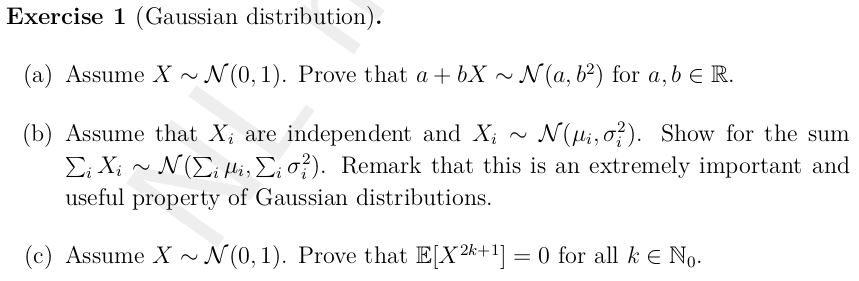
\includegraphics[width=\linewidth]{./exercise1}
	\end{center}
	
	\begin{enumerate}[label=(\alph*), leftmargin=*]
	
	\item
	Wir zeigen hier etwas allgemeiner den Fall einer linearen Transformation einer multivariaten Standardnormalverteilung.
	
	Sei $X \sim \mathcal{N}(0,\one)$. Wir wollen zunächst die Dichte von $Y \defeq H * X$ mit einer invertierbaren Matrix $H \in \R^{n \times n}$ bestimmen. 
	
	Sei dazu $U = H^{-1}$. Wir definieren zu den Matrizen gehörige Abbildungen durch $h({ x})= H { x}$ und $u({ y}) = U { y}$. Schreiben wir $U = \brackets{u_{ij}}_{i,j}$ 
	% und $H = \brackets{h_{ij}}_{i,j}$
	, dann ist $u_i({ y}) = \sum_{i=1}^n u_{ij} y_j$. Es gilt 
	\begin{equation*}
		\frac{\partial u_i}{\partial y_j}= u_{ij}
	\end{equation*}
	und somit ist $J({ y})=U$ die Jacobi-Matrix von $u$. Außerdem gilt
	\begin{equation*}
		\det J({ y})=\det U = \det (H^{-1}) =\frac{1}{\det H} \satzende
	\end{equation*}
	Nutzen wir nun die Transformationsformel für Integrale, so erhalten wir die Dichte
	\begin{align*}
		P({ Y} \in B)&=P(h(X) \in B) \\
		&=P({ X} \in u(B)) \\
		&= \int_{u(B)} (2 \pi)^{-\frac{n}{2}} \exp \left( -\frac{{ x}^\top { x}}{2} \right) \, d { x} \\
		&= \int_{h(u(B))} (2 \pi)^{-\frac{n}{2}} \exp \left( -\frac{u({ y})^\top u({ y})}{2} \right) (\det J({ y})) \, d { y} \\
		&= \int_{B} (2 \pi)^{-\frac{n}{2}} \exp \left( -\frac{(U { y})^\top U { y}}{2} \right) (\det J({ y})) \, d { y} \\
		&= \int_{B} (2 \pi)^{-\frac{n}{2}} \exp \left( -\frac{{ y}^\top U^\top U { y}}{2} \right) \det{U} \, d { y}
	\end{align*}
	Nun wollen wir die Kovarianz von $Y$ bestimmen. Dazu stellen wir fest, dass die Komponenten $X_i$ von $X$ unabhängig sind und somit insbesondere unkorreliert. Außerdem sind sie standardisiert und besitzen somit Kovarianz $1$. Das liefert uns also
	\begin{equation*}
		\Cov(X_i, X_j) = \begin{cases}
		1 & \text{falls } i = j \\
		0 & \text{falls } i \neq j \satzende
		\end{cases}
	\end{equation*}
	Die Kovarianz beschreibt also eine Einheitsmatrix $\one = \Cov(X) =  \brackets{\Cov(X_i, X_j)}_{i,j}$.
	Für die Kovarianz von $Y$ berechnen wir zunächst
	\begin{align*}
		\Cov(Y_i,Y_j)&= \EW[Y_i Y_j] \\
		&= \E\left[ \left( \sum_{a=1}^n H_{ia} X_a \right) \left( \sum_{b=1}^n H_{jb} X_b \right) \right] \\
		&=\sum_{a=1}^n  \sum_{b=1}^n H_{ia} H_{jb} \EW[X_a X_b] \\
		&=\sum_{a=1}^n  \sum_{b=1}^n H_{ia} H_{jb} \Cov( X_a, X_b ) \\
		&=\sum_{a=1}^n H_{ia} H_{ja} \\
		&=(H H^\top)_{ij} \komma
	\end{align*}
	d.h. es gilt $\Cov(Y) = H H^\top$. Schreiben wir nun $\Sigma \defeq \Cov(Y)$ und wollen diese Matrix in der Dichte von $Y$ wiederfinden.
	Diese Dichte haben wir oben berechnet als 
	\begin{equation*}
		(2 \pi)^{-\frac{n}{2}} \exp \left( -\frac{{ y}^\top U^\top U { y}}{2} \right) \det{U}
	\end{equation*}
	mit $U = H^{-1}$. Es gilt
	\begin{equation*}
		U^\top U=(H^{-1})^\top H^{-1} = (H H^\top)^{-1}=\Sigma^{-1}
	\end{equation*}
	und
	\begin{equation*}
		\det U=(\det (U^\top U))^{\frac{1}{2}}=(\det H H^\top)^{-\frac{1}{2}}=(\det \Sigma)^{-\frac{1}{2}} \satzende
	\end{equation*}	
	Damit ist die Dichte von $ Y$ unter Verwendung der Kovarianzmatrix $\Sigma$ gegeben als
	\begin{equation*}
		\frac{1}{\sqrt{(2\pi)^n \det(\Sigma)}} \exp \left( -\frac{{ y}^\top \Sigma^{-1} { y}}{2} \right) \satzende
	\end{equation*}
	
	Verallgemeinern wir dies nun noch auf den Fall einer nicht-zentrierten Zufallsvariable. Dazu definieren wir $Z \defeq H X + \mu$ und $U \defeq H^{-1}$ wie bisher. Damit sind die Abbildungen $u$ und $h$ nun gegeben durch
	\begin{equation*}
		h( x) \defeq H X + \mu \quad \und \quad u( y) \defeq U  (y - \mu) \satzende
	\end{equation*}
	Weiterhin gilt 
	\begin{equation*}
		\brackets{J( y)}_{ij} = \frac{\partial u_i}{y_j} = \sum_{k=1}^n u_{ik} (y_k - \mu_k) = u_{ij} \komma
	\end{equation*}
	d.h. nach wie vor ist $J( y) = U$. Berechnen wir nun analog zu oben die Dichte
	\begin{align*}
		P({ Z} \in B)&=P(h(X) \in B) \\
		&=P({ X} \in u(B)) \\
		&= \int_{u(B)} (2 \pi)^{-\frac{n}{2}} \exp \left( -\frac{{ x}^\top { x}}{2} \right) \, d { x} \\
		&= \int_{h(u(B))} (2 \pi)^{-\frac{n}{2}} \exp \left( -\frac{u({ y})^\top u({ y})}{2} \right) (\det J({ y})) \, d { y} \\
		&= \int_{B} (2 \pi)^{-\frac{n}{2}} \exp \left( -\frac{(U ({ y} - \mu))^\top U ({ y} - \mu)}{2} \right) (\det J({ y})) \, d { y} \\
		&= \int_{B} (2 \pi)^{-\frac{n}{2}} \exp \left( -\frac{({ y} - \mu)^\top U^\top U ({ y} - \mu)}{2} \right) \det{U} \, d { y}
		\satzende
	\end{align*}
	Für den Erwartungswert gilt dann
	\begin{equation*}
		\EW[Z] = \EW[HX + \mu] = H * \EW[X] + \mu = \mu \satzende
	\end{equation*}	
	Damit ist also $Z \defeq HX + \mu$ multivariat normalverteilt mit Erwartungswert $\mu$ und Kovarianzmatrix $\Sigma = HH^\top$.
	
	\item Die momentenerzeugende Funktion einer $\mathcal{N}(\mu_i, \sigma_i^2)$-Verteilung ist gegeben durch
	\begin{equation*}
		m_{X_i}(r) = \exp\brackets{r\mu_i + \frac{r^2 \sigma_i^2}{2}} \satzende
	\end{equation*}
	Aufgrund der Unabhängigkeit der $X_i$ faktorisiert die momentenerzeugende Funktion von $Y \defeq \sum_{i=1}^n X_i$ und wir berechnen
	\begin{equation*}
		\begin{aligned}
			m_Y(r) &= \EW[\exp\brackets{r \sum_{i=1}^n X_i}] = \prod_{i=1} \EW[\exp(X_i)] = \prod_{i=1}^n m_{X_i}(r) = \prod_{i=1}^n \exp\brackets{r\mu_i + \frac{r^2 \sigma_i^2}{2}} \\
			&= \exp\brackets{r \sum_{i=1}^n \mu_i + \frac{r^2 \sum_{i=1}^n \sigma_i^2}{2}} \komma
		\end{aligned}
	\end{equation*}
	was genau der momentenerzeugenden Funktion einer $\mathcal{N}(\sum_{i=1}^n \mu_i, \sum_{i=1}^n \sigma_i^2)$-Verteilung entspricht. Damit ist schließlich $Y \sim \mathcal{N}(\sum_{i=1}^n \mu_i, \sum_{i=1}^n \sigma_i^2)$.
	
	\pagebreak
	
	\item 
	
	Wir betrachten das $k$-te Moment von $X \sim \mathcal{N}(0,1)$
	\begin{equation*}
		\EW[X^k] = \int_\R x^k \frac{1}{\sqrt{2\pi}} \exp\brackets{\frac{x^2}{2}} \dx
	\end{equation*}
	und bezeichnen den Integranten mit $f(x)$. Es gilt 
	\begin{equation*}
		f(-x) = (-x)^k \frac{1}{\sqrt{2\pi}} \exp\brackets{\frac{(-x)^2}{2}} = (-1)^k f(x) \komma
	\end{equation*}
	was für ungerade $k$ schon $f(-x) = -f(x)$ impliziert. Damit muss das Integral gleich Null sein und es gilt $\EW[X^k] = 0$ für alle ungeraden $k$.	
	\end{enumerate}

\end{exercisePage}

\end{document}
